\documentclass[10pt]{beamer}

\usepackage{amsmath,amsthm,amssymb,bm}
\usepackage{xcolor}
\usepackage{cancel}
\usepackage{graphicx}
\usepackage{changepage}
\usepackage{circuitikz}
\usepackage{pgfplots}
\usepackage{physics}
\usepackage{hyperref}
\usepackage{siunitx}
\usepackage{minted}
\usepackage{fontspec}
\usepackage{relsize}
\usepackage{subfig}
\usepackage{mhchem}
\usepackage{todonotes}
\usepackage{biblatex}
\usepackage{multicol, multirow, booktabs}
\usepackage[breakable]{tcolorbox}
% \usepackage[inline]{enumitem}

\pgfplotsset{compat=newest}
\usetikzlibrary{lindenmayersystems}
\usetikzlibrary{arrows}
\usetikzlibrary{calc}
\usetikzlibrary{positioning, fit}
\usetikzlibrary{3d, perspective}
\usetikzlibrary{shapes.geometric}

\definecolor{incolor}{HTML}{303F9F}
\definecolor{outcolor}{HTML}{D84315}
\definecolor{cellborder}{HTML}{CFCFCF}
\definecolor{cellbackground}{HTML}{F7F7F7}
\newcommand{\ui}{\hat{i}}
\newcommand{\uj}{\hat{j}}
\newcommand{\uk}{\hat{k}}
\newcommand{\ux}{\hat{x}}
\newcommand{\uy}{\hat{y}}
\newcommand{\uz}{\hat{z}}
\newcommand{\uv}[1]{\hat{\bm{{#1}}}}
\newcommand{\pr}[1]{{#1^\prime}}
\newcommand{\justif}[2]{&{#1}&\text{#2}}
\newcommand{\dul}[1]{\underline{\underline{#1}}}
\newcommand{\pdiff}[2][]{{\frac{\partial^{#1}}{\partial {{#2}^{#1}}}}}
% \newcommand{\dif}[2][]{{\frac{d^{#1}}{d{{#2}^{#1}}}}}
\pgfdeclarelayer{background}  
\pgfsetlayers{background,main}
\AtBeginDocument{\RenewCommandCopy\qty\SI}

\makeatletter
\newcommand{\boxspacing}{\kern\kvtcb@left@rule\kern\kvtcb@boxsep}
\makeatother
\newcommand{\prompt}[4]{
    \ttfamily\llap{{\color{#2}[#3]:\hspace{3pt}#4}}\vspace{-\baselineskip}
}

\newcommand{\thevenin}[2]{
  \begin{center}
    \begin{circuitikz} \draw
      (0,0) -- (2,0) to[battery1, l_=$V_{Th}\eq#1$] (2,2) 
      to[resistor, l_=$R_{Th}\eq#2$] (0,2)
      ;
      \draw [o-] (-.07,2.079);
      \draw [o-] (-.07,0.079);
    \end{circuitikz}
  \end{center}
}

\newcommand{\norton}[2]{
  \begin{center}
    \begin{circuitikz} \draw
      (0,0) -- (3,0) to[american current source, l_=$I_{N}\eq#1$] (3,2) -- (0,2) (2,0)
      to[resistor, l=$R_{N}\eq#2$] (2,2)
      ;
      \draw [o-] (-.07,2.079);
      \draw [o-] (-.07,0.079);
    \end{circuitikz}
  \end{center}
}

\newcommand{\highlight}[1]{\colorbox{yellow}{#1}}

\newcommand{\ti}[1]{\widetilde{#1}}

\newfontface{\Kaufmann}{Kaufmann}
\DeclareTextFontCommand{\kf}{\Kaufmann}
\newcommand{\scriptr}{\fontsize{12pt}{12pt}\kf{r}}

\newfontface{\KaufmannB}{Kaufmann Bold}
\DeclareTextFontCommand{\kfb}{\KaufmannB}
\newcommand{\bscriptr}{\fontsize{12pt}{12pt}\kfb{r}}

\newcommand{\bv}[1]{\bm{\mathrm{#1}}}

\title{Spontaneous RNA Formation and the First Life on Earth}
\author{Jeremy Favro (0805980) \\ Trent University, Peterborough, ON, Canada}

\begin{document}

\begin{frame}
  \titlepage
\end{frame}
% The formation of biopolymers like RNA and peptides from their constituent monomers in a dilute aqueous
% environment is fundamentally hindered by a significant thermodynamic barrier. This condensation reaction,
% which releases a water molecule for each bond formed, is endergonic (△G∘ > 0) and antientropic (△S∘ < 0), 
% as it combines multiple disordered molecules into a single, more ordered polymer. Consequently, the
% equilibrium in bulk water heavily favors the reverse reaction, hydrolysis, leading to a prevalence of short, non-
% functional oligomers, often termed the Flory Length Problem. However, specific prebiotic environments, such
% as evaporating droplets or surfaces undergoing wet-dry cycles, can invert this unfavorable thermodynamic
% landscape. This process transcends simple concentration effects described by Le Châtelier’s principle; instead,
% it constitutes a form of physical activation. As water evaporates, the increase in the surface-area-to-volume
% ratio forces monomers into a two-dimensional plane, pre-organizing them and mitigating the primary entropic
% penalty of the reaction. This molecular crowding, coupled with the sharply reduced chemical activity of water
% in the nearly-dry state, collectively shifts the reaction’s Gibbs free energy to become exergonic (△G′ < 0).
% This mechanism stands in contrast to chemical activation, which relies on high-energy activating agents (e.g.,
% phosphorimidazolides) to provide the chemical impetus for bond formation.
\begin{frame}
  \frametitle{What am I talking about}
  \begin{columns}
    \begin{column}{0.5\textwidth}
      \begin{itemize}
        \item DNA is made by copying other DNA. RNA is half of DNA
        \item Bootstrap paradox: where did the first DNA come from?
        \item How can we replicate these conditions?
      \end{itemize}
    \end{column}
    % Column 2    
    \begin{column}{0.5\textwidth}
      \begin{figure}
        \centering
        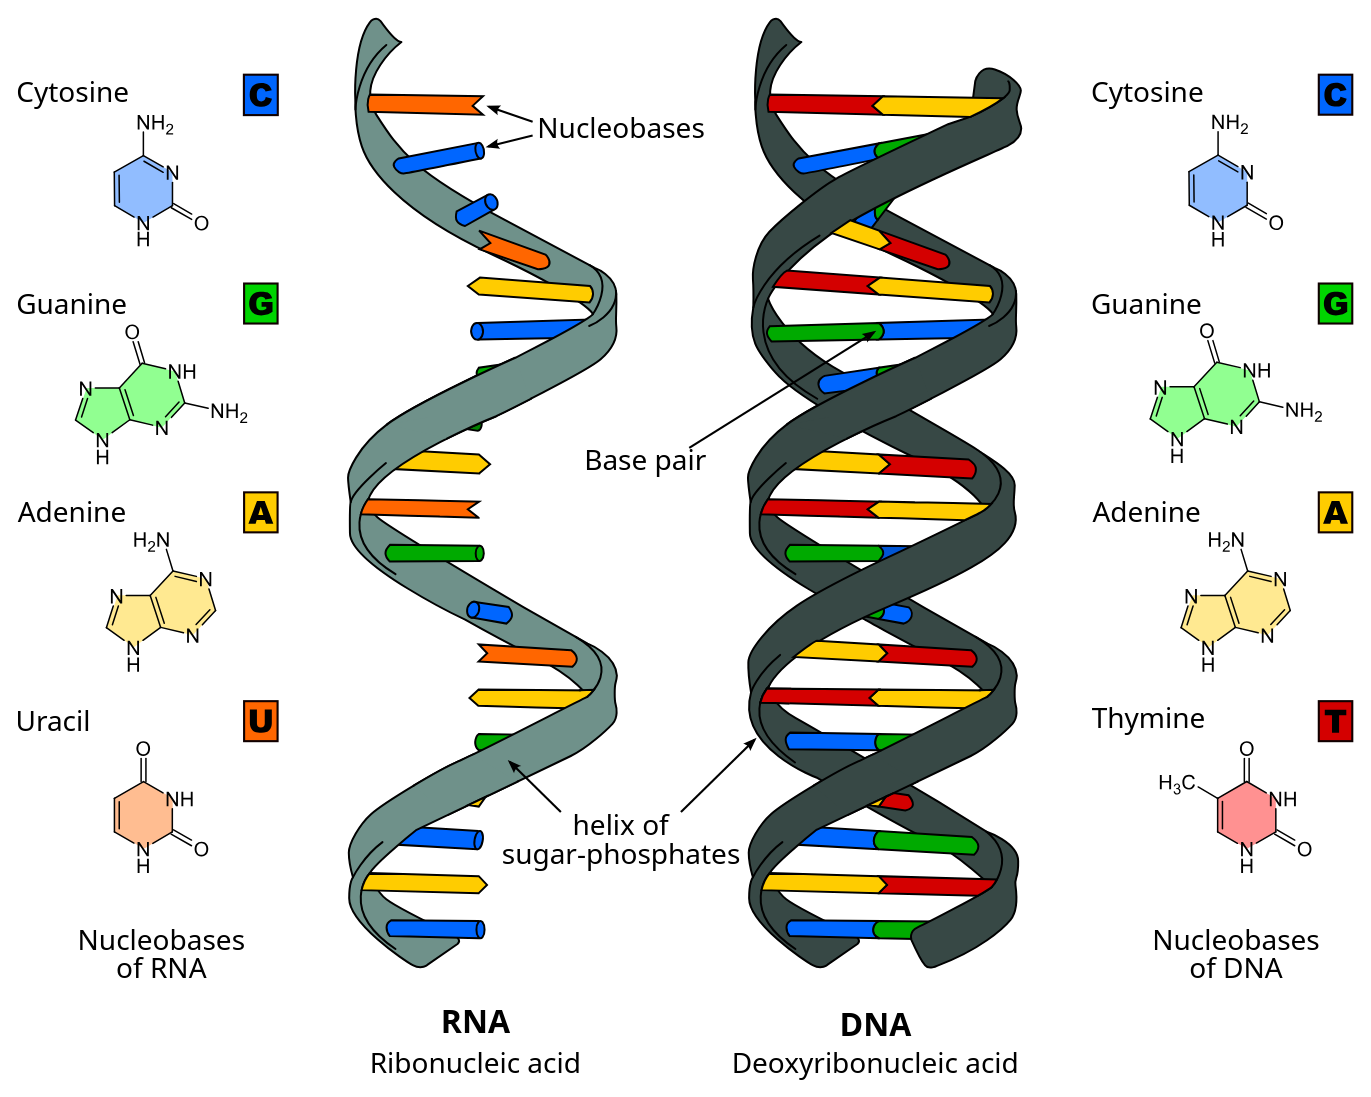
\includegraphics[width=0.8\textwidth]{dna.png}
        \caption{RNA/DNA structures.}
      \end{figure}
    \end{column}
  \end{columns}
\end{frame}

% \begin{frame}
% \frametitle{Table of Contents}
% \tableofcontents
% \end{frame}

\begin{frame}
  \frametitle{Thermodynamic/Energetic Barriers}
  \begin{columns}
    \begin{column}{0.5\textwidth}
      \begin{itemize}
        \item Spontaneous organization of \emph{nucleotides} is limited energetically and physically
        \item Want to bond phosphate-to-phosphate, but they may not be pointed at each other
        \item Also \emph{endergonic}, releases water at every bond formation
        \item Also anti-entropic ($\Delta S < 0$), combining molecules increases order
      \end{itemize}
    \end{column}
    % Column 2    
    \begin{column}{0.5\textwidth}
      \begin{figure}
        \centering
        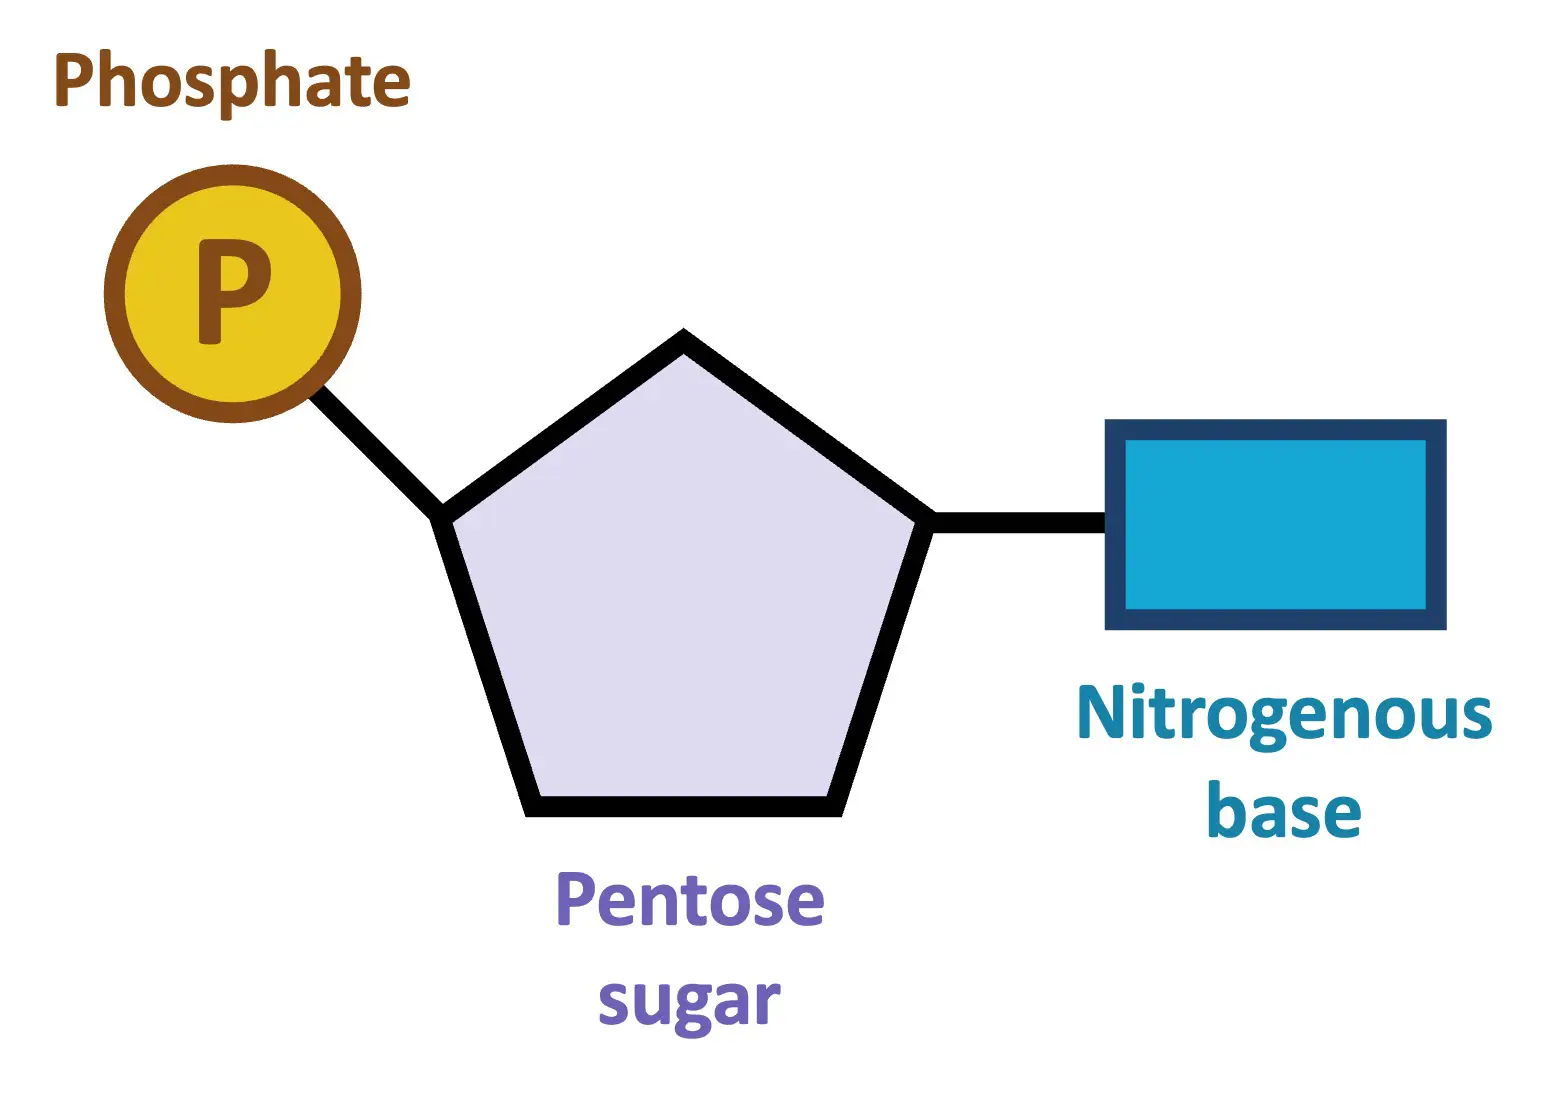
\includegraphics[width=0.7\textwidth]{nucleotide.png}
        \caption{A nucleotide.}
      \end{figure}
    \end{column}
  \end{columns}
\end{frame}

\begin{frame}
  \frametitle{Encouragement}
  \begin{columns}
    \begin{column}{0.5\textwidth}
      \begin{itemize}
        \item Maybe heat? Temperatures required would destroy the nucleotides
        \item Reagents? Unlikely to be responsible for proto-RNA; highly complex chemically
        \item To thermodynamics!
      \end{itemize}
    \end{column}
    % Column 2    
    \begin{column}{0.5\textwidth}
      \begin{figure}
        \centering
        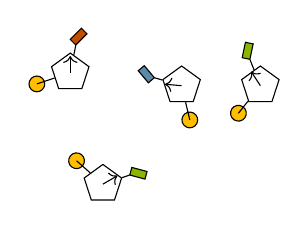
\begin{tikzpicture}
          \definecolor{amber}{rgb}{1.0, 0.75, 0.0}
          \definecolor{airforceblue}{rgb}{0.36, 0.54, 0.66}
          \definecolor{applegreen}{rgb}{0.55, 0.71, 0.0}
          \definecolor{applered}{rgb}{0.75, 0.31, 0.0}

          \begin{scope}[rotate=-15]
            \node[regular polygon, draw, minimum size = 0.5cm] (O) at (0,0) {};
            \draw[->] (0,0) -- ++(0.15,0.15);
            \draw[fill = amber] (O) -- ++(-0.4,0.2) circle (0.1);
            \draw[fill = applegreen] (O) -- ++(0.3,0.2) rectangle ++(0.2, 0.1);
          \end{scope}

          \begin{scope}[xshift=1cm, rotate=45, yshift=2cm]
            \node[regular polygon, draw, minimum size = 0.5cm] (O) at (0,0) {};
            \draw[->] (0,0) -- ++(0.15,0.15);
            \draw[fill = amber] (O) -- ++(-0.4,0.2) circle (0.1);
            \draw[fill = applered] (O) -- ++(0.3,0.2) rectangle ++(0.2, 0.1);
          \end{scope}

          \begin{scope}[xshift=2cm, yshift=1.25cm, rotate=78]
            \node[regular polygon, draw, minimum size = 0.5cm] (O) at (0,0) {};
            \draw[->] (0,0) -- ++(0.15,0.15);
            \draw[fill = amber] (O) -- ++(-0.4,0.2) circle (0.1);
            \draw[fill = applegreen] (O) -- ++(0.3,0.2) rectangle ++(0.2, 0.1);
          \end{scope}

          \begin{scope}[xshift=1cm, yshift=1.25cm, rotate=130]
            \node[regular polygon, draw, minimum size = 0.5cm] (O) at (0,0) {};
            \draw[->] (0,0) -- ++(0.15,0.15);
            \draw[fill = amber] (O) -- ++(-0.4,0.2) circle (0.1);
            \draw[fill = airforceblue] (O) -- ++(0.3,0.2) rectangle ++(0.2, 0.1);
          \end{scope}
        \end{tikzpicture}
        \caption{A bunch of nucleotides whizzing around.}
      \end{figure}
    \end{column}
  \end{columns}
\end{frame}

\begin{frame}
  \frametitle{Constraint}
  \begin{columns}
    \begin{column}{0.5\textwidth}
      \begin{itemize}
        \item We pre-organize the molecules
        \item Force them onto the surface of a sphere
        \item Decreases the Gibbs free energy
              $$G=U+PV-TS$$
              by decreasing degrees of freedom
      \end{itemize}
    \end{column}
    % Column 2    
    \begin{column}{0.5\textwidth}
      \begin{figure}
        \centering
        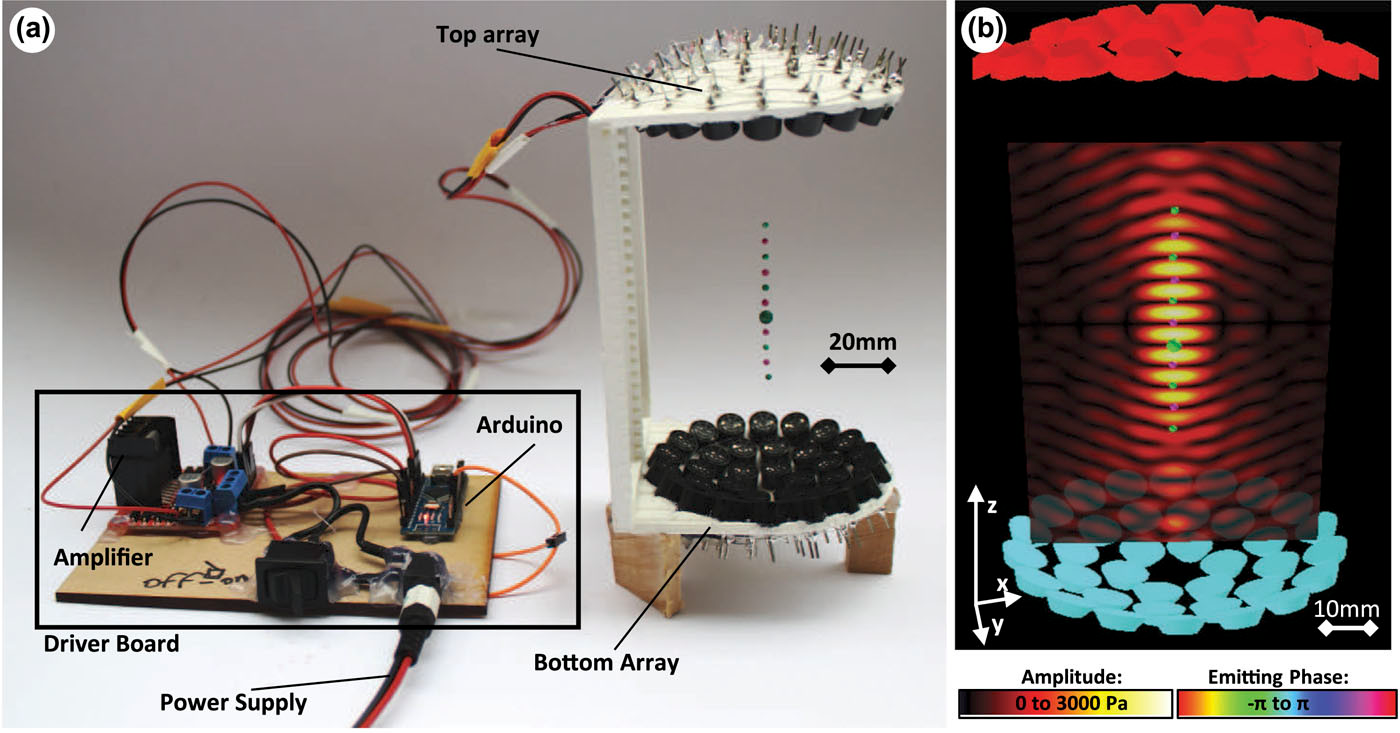
\includegraphics[width=0.8\textwidth]{levitator.png}
        \caption{An ultrasonic levitator.}
      \end{figure}
    \end{column}
  \end{columns}
\end{frame}

\begin{frame}
  \frametitle{Constraint}
  \begin{columns}
    \begin{column}{0.5\textwidth}
      \begin{itemize}
        \item Levitating spheres of nucleotide containing water
        \item Creates a spontaneous reaction, allowing nucleotides to bond
        \item Entirely possible in early-Earth conditions; raindrops, wave spray
      \end{itemize}
    \end{column}
    % Column 2    
    \begin{column}{0.5\textwidth}
      \begin{figure}
        \centering
        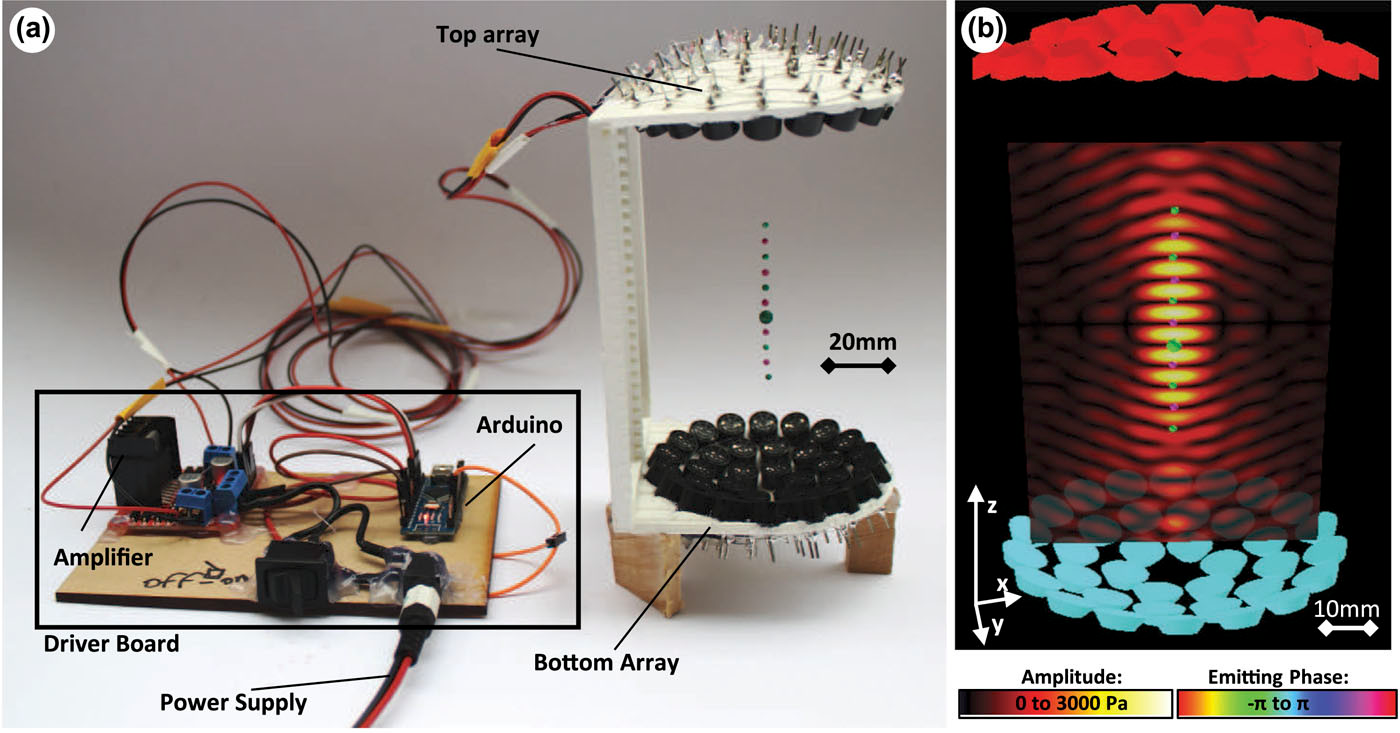
\includegraphics[width=0.8\textwidth]{levitator.png}
        \caption{An ultrasonic levitator.}
      \end{figure}
    \end{column}
  \end{columns}
\end{frame}

\begin{frame}
  \frametitle{Summary}
  \begin{columns}
    \begin{column}{0.5\textwidth}
      \begin{itemize}
        \item Nucleotide bonding into DNA/RNA energetically unfavourable, physically unlikely
        \item Constrain nucleotides to a 2D surface
        \item Enables spontaneous bonding and DNA/RNA formation
        \item Ultrasonic levitators are much less complex than other solutions
      \end{itemize}
    \end{column}

    \begin{column}{0.5\textwidth}
      \begin{figure}
        \centering
        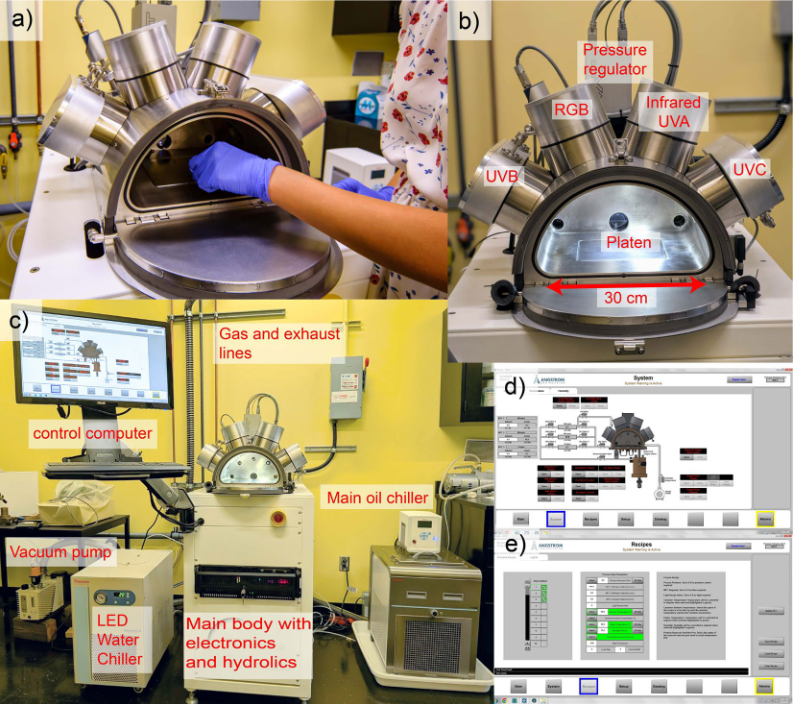
\includegraphics[width=0.8\textwidth]{machine.png}
        \caption{Non-levitating wet-dry cycle device.}
      \end{figure}
    \end{column}
  \end{columns}
\end{frame}
\end{document}